% Full-width TikZ overview shared by the Elsevier and IEEE entry points.
\usetikzlibrary{arrows.meta,positioning}

\begin{figure*}[!t]
\centering
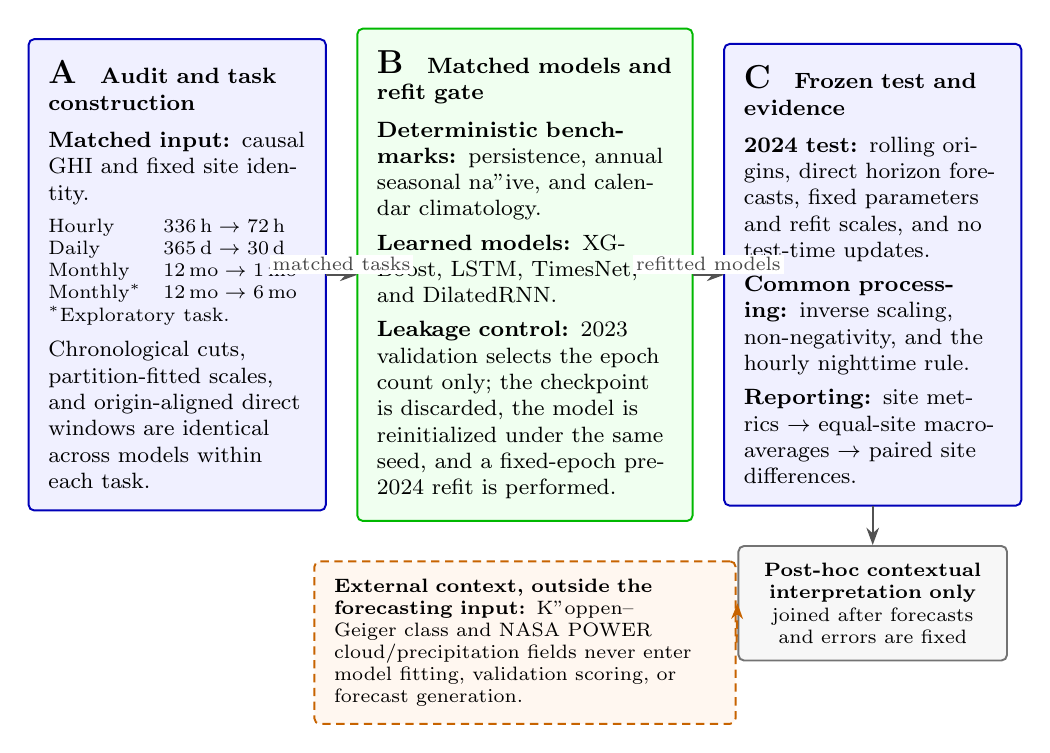
\begin{tikzpicture}[
  font=\footnotesize,
  stage/.style={
    draw=#1!72!black,
    fill=#1!6,
    rounded corners=2pt,
    line width=0.7pt,
    align=left,
    inner xsep=2.5mm,
    inner ysep=2.8mm,
    outer sep=0pt
  },
  flow arrow/.style={
    -{Stealth[length=2.2mm,width=1.6mm]},
    draw=black!68,
    line width=0.8pt
  },
  arrow label/.style={
    fill=white,
    inner sep=1pt,
    font=\scriptsize,
    text=black!72
  },
  external/.style={
    draw=orange!78!black,
    fill=orange!6,
    densely dashed,
    rounded corners=2pt,
    line width=0.7pt,
    align=left,
    inner xsep=2.5mm,
    inner ysep=2.2mm,
    font=\scriptsize
  },
  posthoc/.style={
    draw=black!55,
    fill=black!3,
    rounded corners=2pt,
    line width=0.7pt,
    align=center,
    inner xsep=2.5mm,
    inner ysep=2.2mm,
    font=\scriptsize
  }
]

\node[stage=blue,text width=0.27\textwidth] (stage-a) {
  {\large\bfseries A}\quad\textbf{Audit and task construction}\\[1.4mm]
  \textbf{Matched input:} causal GHI and fixed site identity.\\[1.2mm]
  {\scriptsize
  \begin{tabular}{@{}l@{\quad}l@{}}
    Hourly & $336\,\mathrm{h}\rightarrow72\,\mathrm{h}$ \\
    Daily & $365\,\mathrm{d}\rightarrow30\,\mathrm{d}$ \\
    Monthly & $12\,\mathrm{mo}\rightarrow1\,\mathrm{mo}$ \\
    Monthly$^{\ast}$ & $12\,\mathrm{mo}\rightarrow6\,\mathrm{mo}$
  \end{tabular}}\\[-0.2mm]
  {\scriptsize $^{\ast}$Exploratory task.}\\[1.2mm]
  Chronological cuts, partition-fitted scales, and origin-aligned direct
  windows are identical across models within each task.
};

\node[stage=green,text width=0.31\textwidth,right=4mm of stage-a] (stage-b) {
  {\large\bfseries B}\quad\textbf{Matched models and refit gate}\\[1.4mm]
  \textbf{Deterministic benchmarks:} persistence, annual seasonal na"ive,
  and calendar climatology.\\[1.0mm]
  \textbf{Learned models:} XGBoost, LSTM, TimesNet, and DilatedRNN.\\[1.0mm]
  \textbf{Leakage control:} 2023 validation selects the epoch count only;
  the checkpoint is discarded, the model is reinitialized under the same
  seed, and a fixed-epoch pre-2024 refit is performed.
};

\node[stage=blue,text width=0.27\textwidth,right=4mm of stage-b] (stage-c) {
  {\large\bfseries C}\quad\textbf{Frozen test and evidence}\\[1.4mm]
  \textbf{2024 test:} rolling origins, direct horizon forecasts, fixed
  parameters and refit scales, and no test-time updates.\\[1.0mm]
  \textbf{Common processing:} inverse scaling, non-negativity, and the hourly
  nighttime rule.\\[1.0mm]
  \textbf{Reporting:} site metrics $\rightarrow$ equal-site macro-averages
  $\rightarrow$ paired site differences.
};

\draw[flow arrow] (stage-a.east) --
  node[arrow label,above] {matched tasks} (stage-b.west);
\draw[flow arrow] (stage-b.east) --
  node[arrow label,above] {refitted models} (stage-c.west);

\node[external,text width=0.40\textwidth,below=5mm of stage-b] (external-data) {
  \textbf{External context, outside the forecasting input:}
  K"oppen--Geiger class and NASA POWER cloud/precipitation fields never enter
  model fitting, validation scoring, or forecast generation.
};

\node[posthoc,text width=0.24\textwidth,below=5mm of stage-c] (interpretation) {
  \textbf{Post-hoc contextual interpretation only}\\
  joined after forecasts and errors are fixed
};

\draw[flow arrow] (stage-c.south) -- (interpretation.north);
\draw[-{Stealth[length=2.0mm,width=1.5mm]},densely dashed,
      draw=orange!78!black,line width=0.75pt]
  (external-data.east) -- (interpretation.west);

\end{tikzpicture}
\caption{Unified multi-resolution pipeline. The four frozen task contracts are
evaluated on matched origins across deterministic benchmarks and learned
models. External climate and weather products are excluded from model inputs
and enter only after forecasts and errors are fixed. Algorithms~\ref{alg:block_a}--
\ref{alg:block_c} provide the corresponding pseudocode.}
\label{fig:pipeline}
\end{figure*}
